

\section{Introduction}
\begin{figure*}[t]
\centering
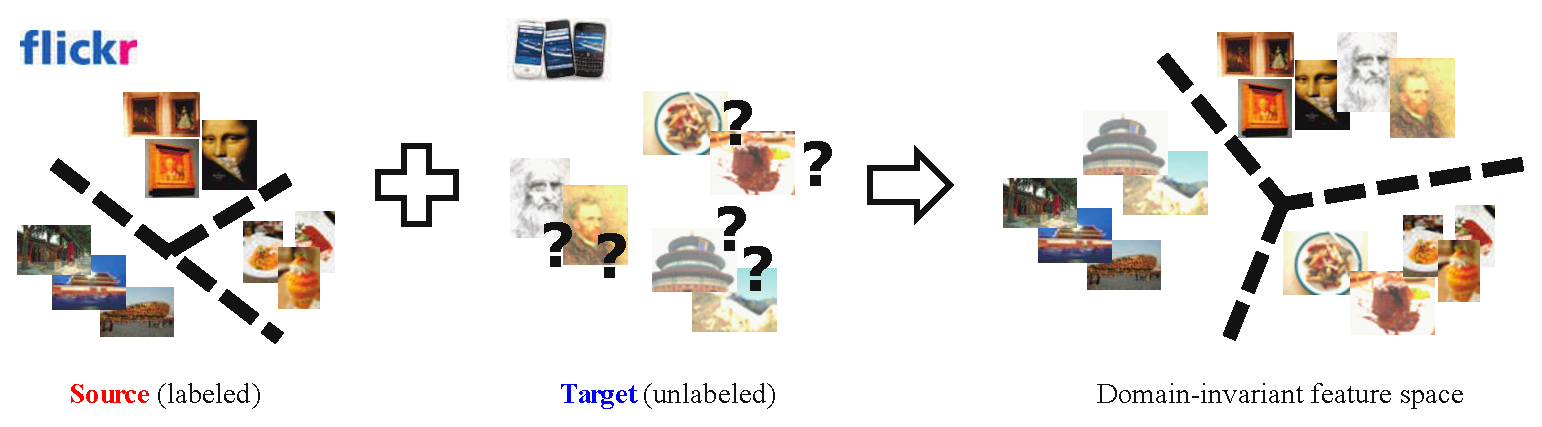
\includegraphics[width=0.92\columnwidth]{fig/fImageConcept_3.eps}
\caption{An illustrative example of {\bf unsupervised domain adaptation}. The goal is to classify unlabeled data from the \blue{target} domain that has different characteristics from the \red{source} domain where annotated data are provided. The central idea behind our approaches is to use the data from both domains to infer a domain-invariant feature/kernel space such that, in this space, the classifier learned using the labels of the source domain will likely work well on the target domain.}
\label{fConceptUDA}
\end{figure*}

Statistical machine learning algorithms often rely on the assumption that data used for training and testing are drawn from the same distribution. However, the validity of this assumption is frequently challenged in real-world applications. Figure~\ref{fConceptUDA} gives an illustrative example. Imagine that we are to deploy an APP to recognize images captured by mobile phone cameras. Instead of demanding that users provide labels to our learning algorithms, can we train classifiers with existing tagged Flickr images, and hope the classifiers will still work well on mobile camera test images? Our intuition says no. We suspect that the strong distinction between the Flickr images and the typical mobile phone images will cripple the classifiers.

Indeed, a stream of studies has shown that when the classifiers for object recognition are evaluated outside of their training datasets, the performance degrades significantly~\cite{TorralbaCVPR11Unbiased,DollarCVPR09Pedestrian,PerronninCVPR10Largescale}.  The culprit is clear: the visual appearance  of even the same object varies across different datasets as a result of many factors, such as imaging devices, photographers' preferences, and background. These idiosyncrasies often cause a substantial mismatch between the training and testing data. In addition to object recognition, the mismatch is also abundant in other computer vision tasks~\cite{DuanCVPR09Domain,WangCVPR2011automatic,JainCVPR10online,DuanPAMI12Visual}, speech recognition~\cite{LeggetterCSL95Maximum}, and text analysis~\cite{BlitzerACL07domain,BlitzerEMNLP06Domain}. 






In all these pattern recognition tasks, there is a common theme. There are  two distinct types of datasets: one from a \textbf{source} domain and the other from a \textbf{target} domain. The source domain contains a large amount of labeled data such that a classifier can be reliably built. The target domain refers broadly to a related dataset that has different characteristics compared to the source domain.  In other words, the underlying distributions of the datasets are different. Note that we assume the set of possible labels remains the same across domains.



%Thus, the main objective is to \emph{adapt} classifiers trained on the source domain to the target domain to attain good performance there.

\subparagraph{How to build classifiers that are robust to the mismatched distributions?}
Techniques for addressing this challenge have been  investigated under the names of domain adaptation, covariate shift, or  transfer learning~\cite{shimodaira00shift,daume06domain,pan2009survey,gretton09kmm}. When there is no labeled data from the target domain to help learning, the problem, illustrated in Fig.~\ref{fConceptUDA},  is called \textbf{{unsupervised domain adaptation}}~\cite{BlitzerACL07domain,BlitzerEMNLP06Domain,gopalan2011domain,gong12gfk,chen11cotrain}. When some labeled  data from the target domain is accessible (but insufficient for constructing a good classifier), the problem is similar to semi-supervised learning and is named semi-supervised domain adaptation \cite{daume10co,bergamo09weak,saenko2010adapting}. In either case, how to effectively leverage \emph{unlabeled} target data is key to domain adaptation.


%We focus on unsupervised domain adaptation in this chapter as it is highly desirable in real-world applications. It taxes users minimally, as the recognition system adapts automatically. While appealing, unsupervised domain adaptation is especially challenging. For example, the common practice of discriminative training is generally not applicable. Without labels, it is not even clear how to define the right discriminative loss on the target domain! Similarly, it is also difficult to perform model selection.% (e.g., tuning regularization coefficients).

%We focus on overcoming those challenges.  Our core idea is to model how the source and target are related in order to enable unsupervised domain adaptation. Our effort centers around the notion of learning kernel functions as a way to infer robust features that are resilient (``invariant") to the mismatch between domains.

Discovering domain-invariant feature spaces that enable the adaptation of classifiers or regressors has been an extensively studied paradigm~\cite{bendavid07domain,BlitzerEMNLP06Domain,BlitzerACL07domain,daume07easy,tca}. The feature representation can be derived using auxiliary tasks that predict ``pivot features''~\cite{ando05,BlitzerEMNLP06Domain}, augmenting the feature space~\cite{daume07easy,daume10co,li2012discriminative,gopalan2013learning}, co-training with multi-view representations~\cite{chen11cotrain}, or matching probabilistic distributions~\cite{tca}. In a such space, the source and target domains have the same (or similar) marginal distributions over the input data, and the posterior distributions of the labels are often assumed to be the same across domains too. Hence, a conventional classifier trained on the labeled source would  likely  perform  well on the target. Some theoretical analyses show that the generalization capability of the classifier on the target is indeed positively correlated with the domain-invariance, measured by different metrics, of the learned feature spaces~\cite{BenDavid10Adaptation,mansour09domain,mansour09multiple}.

Many existing feature learning methods in domain adaptation, however, are not directly applicable to {\em visual recognition}. For instance, the bag-of-words representations in natural language process often contain semantic and discriminative ``pivot'' features that transfer across domains~\cite{daume07easy,BlitzerEMNLP06Domain,BlitzerACL07domain,chen11cotrain}; to determine the sentiments (\textsc{positive} versus \textsc{negative}) of consumers' product reviews, words like ``do not buy'' transcend product categories. In computer vision tasks, this intuition no longer holds. Often, no single feature  is discriminative enough for visual recognition tasks.

\subparagraph{How can we infer an invariant feature space from \emph{visual} data?} 

We therefore propose novel approaches to unsupervised domain adaptation, with applications to visual recognition in mind. We focus on unsupervised domain adaptation as it is highly desirable in real-world applications. It taxes users minimally by automatically adapting the visual recognition systems. While appealing, unsupervised domain adaptation is especially challenging. For example, the common practice of discriminative training is generally not applicable. Without labels, it is not even clear how to define the right discriminative loss on the target domain! Similarly, it is also difficult to perform model selection.% (e.g., tuning regularization coefficients).

We overcome those challenges by leveraging the conceptual connection between features and kernels, in order to better relate the source and target domains. Instead of explicitly defining which features are domain-invariant, we discover them \emph{implicitly} by learning kernel functions that compute the inner products between data points in a (transformed) feature space. Thus, inferring domain-invariant feature spaces is equivalent to learning kernel functions that ``host'' those features.

Learning kernels has been employed in a variety of problems in computer vision and machine learning~\cite{lanckriet04kernel,mkl_obj,ham2004kernel,roweis2000nonlinear,weinberger2006unsupervised}. As our ultimate goal is to build a classifier that performs well on the target, the framework of discriminatively combining multiple kernels is especially appealing~\cite{lanckriet04kernel}. To this end, we need address two crucial and interdependent questions: what to use as base kernels, and how to discriminatively combine them when there is no labeled data from the target domain?  

Our solution rests on two novel modeling considerations in a seamless fashion. The first  leads to the development of the {\bf geodesic flow kernel (GFK)}~\cite{GongCVPR12Geodesic}, and is based on the idea of intermediate feature spaces. Analogous to unsupervised manifold learning of kernels, GFK exploits the structures of low-dimensional subspaces in visual data. It measures the data pairwise similarities that are insensitive to variations in domains. In particular, it results from aggregating the inner products computed within a sequence of infinite subspaces interpolating between the source and target domains. While each subspace may idiosyncratically favor the source or the target domain, the aggregation smooths out the idiosyncrasies. Consequently, when used in a nearest neighbor classifier as a similarity measure, GFK outperforms many competing methods for domain adaptation. The kernel function can be computed without requiring any labels from the target domain and can be plugged into any kernel-based classifier. We present the details in section~\ref{sGFK}. 

Our second modeling consideration aims to further improve GFK's discriminative power, centering around the notion of \textbf{landmarks}~\cite{GongICML13Connecting}. Concretely, we exploit the insight that \emph{not all instances from the source domain are created equally in terms of adaptability}~\cite{GongICML13Connecting}.  Existing research in modeling the discrepancy between domains has been limited to macroscopically examining their distribution similarity by tuning to statistical properties of the samples as a whole --- when comparing (marginal) distributions to derive features, all the samples are used. This notion  is stringent, as it requires all discrepancies to  be accounted for and forces learning inefficiently (or even erroneously) from ``hard'' cases that might be just outliers to the target domains (cf.\ examples in Fig.~\ref{fLandmark}).

In contrast, we examine distribution similarity microscopically at the instance level.  Our approach automatically plucks out and exploits the most desirable {\bf ``landmark"} instances from the source domain. The landmarks bridge the source and the target domains at a fine granularity; they are labeled instances from the source domain that are distributed similarly to the target domain. As a result, the labels of the landmarks serve as a good proxy for us to approximate the discrimintive loss on the target domain. We show how to use those landmarks to construct multiple domain-invariant features (i.e., multiple GFKs) and how those kernels can be discriminatively combined to learn a new domain-invariant feature space such that the adapted classifier performs the best on the target domain  (cf.\ section~\ref{sLandmark}).


We conduct extensive empirical studies to validate our approaches on the task of visual object recognition, where we train classifiers on one dataset and then apply them to others (section~\ref{sExp}). Section~\ref{sConclusion} concludes this chapter. 


\section{Learning kernels for unsupervised domain adaptation}
This section presents our kernel approach to unsupervised domain adaptation. We first derive the base geodesic flow kernels that entail domain-invariant features and infinite subspaces between the source and target domains, and then develop the landmark based algorithm to combine the base kernels with approximated discriminative loss of the target. Our emphasis on the kernel learning aspect sheds light on future research. We believe the core paradigm of learning invariant features for domain adaptation can be further advanced by a broader set of kernel  techniques. 


\eat{
{\bf Contributions.} 
Our main contributions lie in developing new kernel learning methods for unsupervised domain adaptation and validating their effectiveness in object recognition. Our emphasis on the kernel learning aspect not only provides a natural connection between our two approaches, GFK~\cite{GongCVPR12Geodesic} and the landmark-based domain adaptation~\cite{GongICML13Connecting}, but also sheds light on future research directions. Specifically, we believe the core paradigm of learning invariant feature spaces can be further advanced by a broader set of kernel learning techniques.  %In addition, we present significantly more details on our empirical studies and an improved exposition of key ideas and algorithms. 


In section~\ref{sGFK}, we derive our \textbf{geodesic flow kernel (GFK)} --- a kernel function that exploits intrinsic low-dimensional subspaces in visual data and measures similarity using those subspaces. The kernel function can be computed without requiring any labels from the target domain and can be plugged into any kernel-based classifier. Furthermore, using the kernel avoids cross-validation of hyperparameters.

In section~\ref{sLandmark}, we develop an approach that further improves GFK's discriminative power. The  approach centers around the notion of \textbf{landmarks}. Landmarks reveal domain similarity at a fine granularity; they are defined as a subset of labeled instances from the source domain that are distributed similarly to the target domain. Thus, they are expected to function as a conduit \emph{connecting} the source and target domains to facilitate adaptation. We show how to use those landmarks to construct multiple domain-invariant features (i.e., multiple GFKs) and how those kernels can be discriminatively combined to learn a new domain-invariant feature space such that the adapted classifier performs the best on the target domain.

}
